\chapter{Hardware Development}

One of the cornerstones of our team's Concept of Operations for the SubT Challenge was modular autonomy. That is, we wanted to develop a series of modules which could be composed and rapidly reconfigured to suit the task at hand. The use of individual modules would also allow for components to be replaced or upgraded as necessary. For example, each of our ground robots had 4 drive modules, each consisting of a wheel, motor, gearbox, and a separate electronics module. The drive modules could be replaced or upgraded as necessary, such as in the case of a gearbox failing or the selection of different desired torque profiles. Similarly, we wanted to develop modular sensing and compute payloads which could be transferred across different robots, including in between ground and aerial robots, and which would be capable of performing all of the robot's high level autonomy functions.

Early indication that our approach should be feasible came as the result of using a prototype state estimation payload ("Blue Payload") similar to the Kaarta Traak \cite{kaarta_traak}. The payload was relatively small, self-contained, and could be easily transferred between robots (see Figure \ref{blue payload robots}). We simply had to mount the payload to the robot, apply power, and connect to the robot's internal network, and all of the payload's autonomy functions would be enabled. Overall, we found the Blue Payload quite simple to integrate, and wanted our future payloads to be similar in this regard. Inspired by the Blue Payload, and keeping the SubT Challenge requirements and timeline in mind, we came up with a list of some design goals and desired capabilities for our first payload:

\begin{description}
	\item[Self-contained] All of the sensing and computation for the high level autonomy features should happen inside the payload itself. Ideally, the payload would only be supplied power and a network connection, just like the Blue Payload, and would output autonomy goals (such as waypoints) and information (such as robot state, maps, and artifact locations) to be relayed to the human supervisor at the base station.
	\item[Environmentally Robust] We expected the field environments for the SubT competition to be somewhat hostile to the sensors. Specifically, we were told that "dust, fog, mist, water, and smoke are within scope" \cite{tunnel_rules}, and we wanted our payload to be reasonably protected against these elements, within reason. Additionally, the payload needed to be robust to the mechanical loading it would be subject to as a result of the rough terrain.
	\item[Low Cost] While there aren't specific restrictions on the maximum cost of our robot, DARPA was interested in identifying cost effective solutions for the SubT Challenge. Minimizing cost is also useful as a design goal as we intended to build multiple copies of the payload for our various robots, as well as to have spares.
	\item[Weight Sensitivity] Similar to the Blue Payload, we wanted our new payload to be light enough to be carried by one of our aerial robots (as in Figure \ref{d1 blue payload}), or a smaller ground robot (as in Figure \ref{joeybot blue payload}) in addition to larger robots (as in Figure \ref{r1 blue payload}).
	\item[Rapid Development] From the beginning of the competition (September 2018) to the first qualification deadline (December 2018), we had a little under 3 months to develop our first payload. This meant that, wherever possible, we should prefer designs that relied on existing expertise, such as the use of familiar components and sensors, and preferring in-house manufacturing capabilities with short lead times.
\end{description}

\begin{figure}
	\centering
	\begin{subfigure}{0.3\textwidth}
		\includegraphics[width=\textwidth]{blue_payload_joeybot.png}
		\caption{Joeybot with Blue Payload}
		\label{joeybot blue payload}
	\end{subfigure}		
	\hfill
	\begin{subfigure}{0.3\textwidth}
		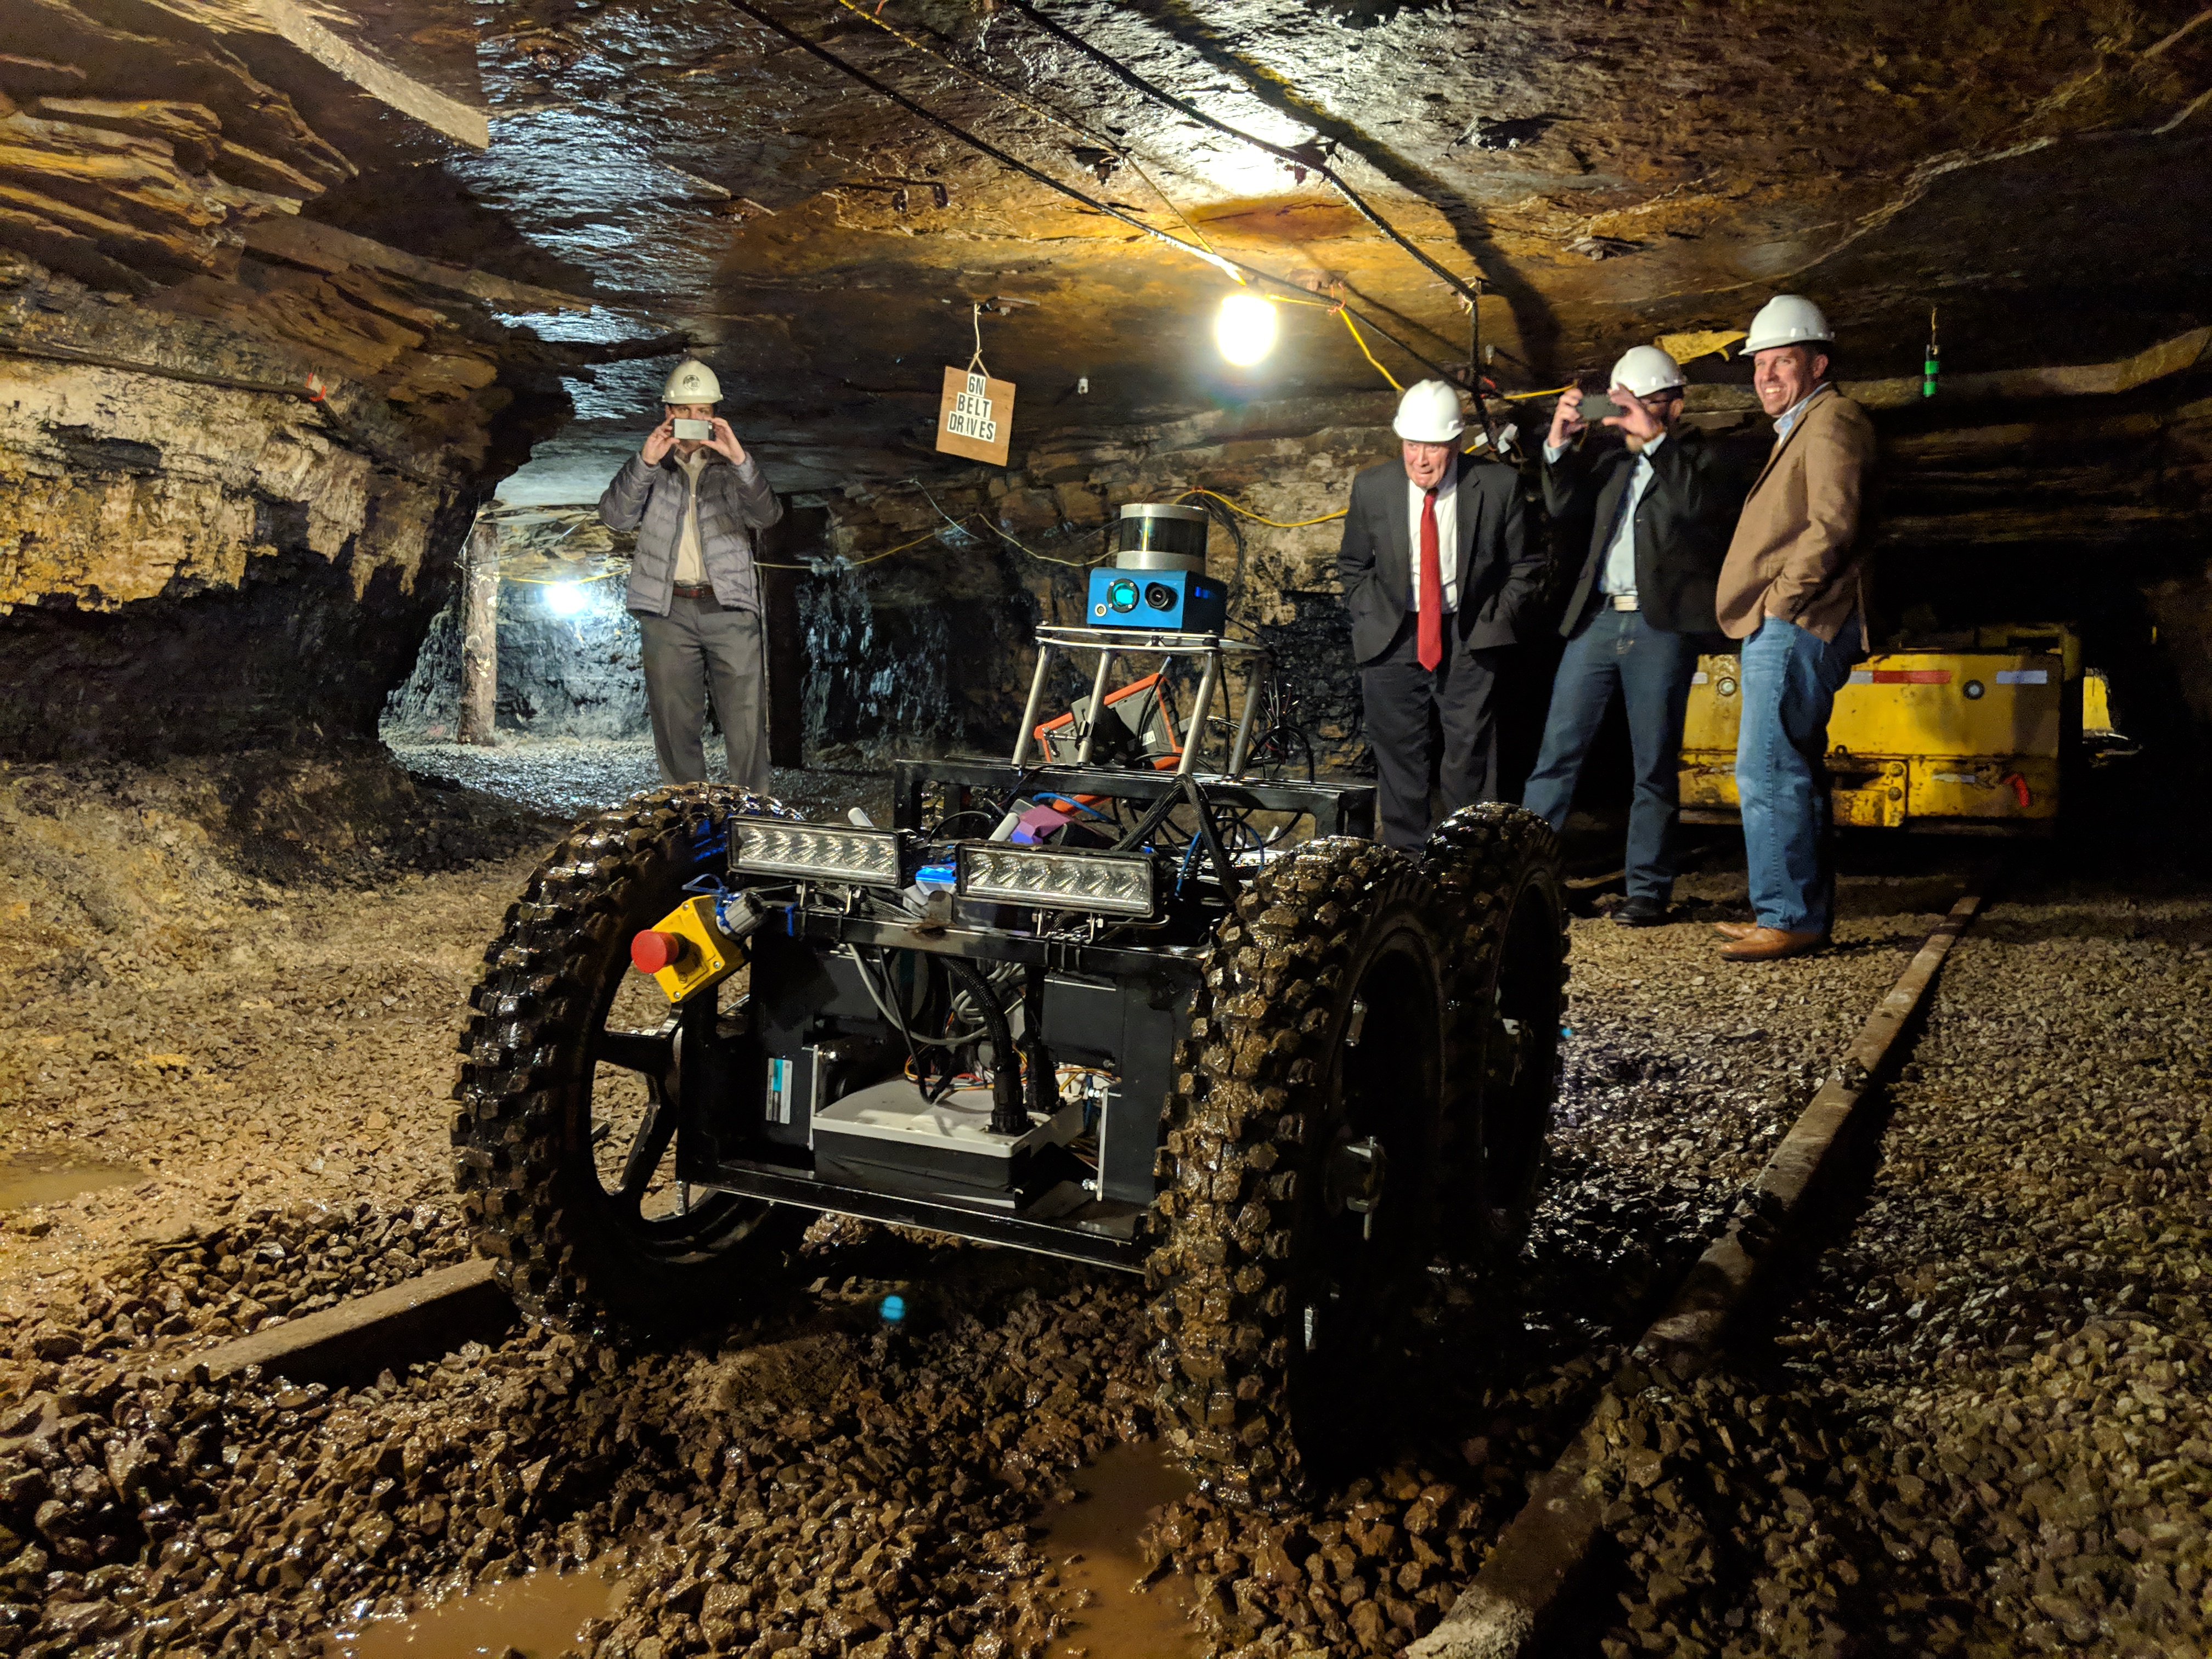
\includegraphics[width=\textwidth]{r1_with_blue_payload.jpg}
		\caption{R1 with Blue Payload}
		\label{r1 blue payload}		
	\end{subfigure}
	\hfill
	\begin{subfigure}{0.3\textwidth}
		\includegraphics[width=\textwidth]{drone_with_blue_payload.png}
		\caption{D1 with Blue Payload}
		\label{d1 blue payload}
	\end{subfigure}	
	\caption{Robots with initial modular payload ("Blue Payload")}
	\label{blue payload robots}
\end{figure}

\begin{enumerate}
	\item Computers (for both object detection and SLAM)
	\item Sensing (both for SLAM and object detection), as well as sensor placement 
	\item sensor synchronization (maybe not its own bullet?)
	\item power management / distribution (everything in the box should be powered by a single cable)
	\item connectors (internal and external) (including debugging)
	\item heat dissipation (more of a mechanical problem)
	\item mounting
\end{enumerate}